\documentclass[a4paper, 11pt, oneside, oldfontcommands]{memoir}

%%%%% Packages %%%%%
\usepackage{lmodern}
\usepackage{palatino}
\usepackage[T1]{fontenc}
\usepackage[utf8]{inputenc}
\usepackage[french]{babel}


%%%%%%%%%%%%%%%%%%%%  PACKAGE SECONDAIRE

%\usepackage{amstext,amsmath,amssymb,amsfonts} % package math
%\usepackage{multirow,colortbl}	% to use multirow and ?
%\usepackage{xspace,varioref}
\usepackage[linktoc=all, hidelinks]{hyperref}			% permet d'utiliser les liens hyper textes
\usepackage{float}				% permet d ajouter d autre fonction au floatant
%\usepackage{wrapfig}			% permet d avoir des image avec texte coulant a cote
%\usepackage{fancyhdr}			% permet d inserer des choses en haut et en bas de chaque page
\usepackage{microtype}			% permet d ameliorer l apparence du texte
\usepackage[explicit]{titlesec}	% permet de modifier les titres
\usepackage{graphicx}			% permet d utiliser les graphiques
\graphicspath{{./img/}}		% to say where are image
%\usepackage{eso-pic} 			% to put figure in the background
\usepackage[svgnames]{xcolor}	% permet d avoir plus de 300 couleur predefini
%\usepackage{array}				% permet d ajouter des option dans les tableaux
%\usepackage{listings}			% permet d ajouter des ligne de code
%\usepackage{tikz}				% to draw figure
%\usepackage{appendix}			% permet de faire les index
%\usepackage{makeidx}			% permet de creer les index
%\usepackage{fancyvrb}			% to use Verbatim
%\usepackage{framed}				% permet de faire des environnement cadre
%\usepackage{fancybox}			% permet de realiser les cadres
\usepackage{titletoc}			% permet de modifier les titres
%\usepackage{caption}
\usepackage[a4paper, top=2cm, bottom=2cm]{geometry}
\usepackage{frbib}                      %permet d avoir une biblio francaise
\usepackage[babel=true]{csquotes}


\usepackage{graphicx}
\RequirePackage{pageGardeEnsta}	% permet d avoir la page de garde ensta

%\setcounter{secnumdepth}{2}		% permet d'augmenter la numerotation
%\setcounter{tocdepth}{2}		% permet d'augmenter la numerotation

%%%%%%%%%%%%%%%%%%  DEFINITION DES BOITES
\newcounter{rem}[chapter]

\newcommand{\remarque}[1]{\stepcounter{rem}\noindent\fcolorbox{OliveDrab}{white}{\parbox{\textwidth}{\textcolor{OliveDrab}{
\textbf{Remarque~\thechapter.\therem~:}}\\#1}}}

\newcounter{th}[chapter]

\newcommand{\theoreme}[2]{\noindent\fcolorbox{FireBrick}{white}{\stepcounter{th}
\parbox{\textwidth}{\textbf{\textcolor{FireBrick}{Théorème~\thechapter.\theth~:}}{\hfill \textit{#1}}\\#2}}}

\newcommand{\attention}[1]{\noindent\fcolorbox{white}{white}{\parbox{\textwidth}{\textcolor{FireBrick}{
\textbf{Attention !}}\\\textit{#1}\\}}}
%%%%%%%%%%%%%%%%%%%%%%%%%%%%%%%%%%%%%%%%%%%%%%%%%%%%%%%%%%%%%%%%%%%%%%%%%


%% INDEX %%%%%%%%%%%%%%%%%%%%%%%%%%%%%%%%%%%%%%%%%%%%%%%%%%%%
\makeindex

%%%%% Useful macros %%%%%
\newcommand{\latinloc}[1]{\ifx\undefined\lncs\relax\emph{#1}\else\textrm{#1}\fi\xspace}
\newcommand{\etc}{\latinloc{etc}}
\newcommand{\eg}{\latinloc{e.g.}}
\newcommand{\ie}{\latinloc{i.e.}}
\newcommand{\cad}{c'est-à-dire }
\newcommand{\st}{\ensuremath{\text{\xspace s.t.\xspace}}}
\newcommand{\aes}{AES-GCM }

%%%% Definition des couleur %%%%

\newcommand\couleurb[1]{\textcolor{SteelBlue}{#1}}
\newcommand\couleurr[1]{\textcolor{DarkRed}{#1}}


%% number page style style %%%%%%%%%%%%%%%%%%%%%%%%%%%%%%%%%%%%%%%%%%%%%%%%%%%%%%

\pagestyle{plain}
%\pagestyle{empty}
%\pagestyle{headings}
%\pagestyle{myheadings}



%% chapters style %%%%%%%%%%%%%%%%%%%%%%%%%%%%%%%%%%%%%%%%%%%%%%%%%%%%%%
%% You may try several styles (see more in the memoir manual).

%\chapterstyle{veelo}
%\chapterstyle{chappell}
%\chapterstyle{ell}
%\chapterstyle{ger}
%\chapterstyle{pedersen}
%\chapterstyle{verville}
\chapterstyle{madsen}
%\chapterstyle{thatcher}


%%%%% Report Title %%%%%
\title{AES-GCM}
\author{\textsc{Rigaud Michaël} et \textsc{Badier Charlie}}
\date{\today}
\doctype{UV4.8}
\promo{promo 2017}
\etablissement{\textsc{Ensta} Bretagne\\2, rue François Verny\\
  29806 \textsc{Brest} cedex\\\textsc{France}\\Tel +33 (0)2 98 34 88 00\\ \url{www.ensta-bretagne.fr}}
\logoEcole{
\includegraphics[height=4.2cm]{logo_ENSTA_Bretagne_Vertical_CMJN}}



%%%%%%%%%%%%%%%%%% DEBUT DU DOCUMENT
\begin{document}

\maketitle
\thispagestyle{empty}
\newpage

\tableofcontents


%%%%%%%%%%%%%%%%% INTRODUCTION

\chapter*{Introduction}
\addcontentsline{toc}{chapter}{Introduction}

GCM ou Galois Counter Mode est un mode d'opération de chiffrement par bloc en cryptographie symétrique. C'est un algorithme de chiffrement authentifié qui garanti l'intégrité et l'authenticité des données. Lors des opérations que nous verrons plus loin, cet algorithme demande de chiffrer avec un autre algorithme de chiffrement. D'après la norme IEEE 802.1AE, on utilise l'algorithme AES (Advanced Encryption Standard). On appelle donc cet algorithme \aes.

Dans ce rapport, nous expliquerons dans un premier temps le fonctionnement de \aes ainsi que de ses autres modes. Puis nous le comparerons à d'autres algorithmes semblables en termes de complexité. Enfin, nous essayerons de voir quels sont les principaux vecteurs d'attaques de cet algorithme dans les applications usuelles.


\newpage	  
%%%%%%%%%%%%%%%%%%%%%%%%

\chapter{Différents modes de fonctionnement cryptographique}
\label{chap:différents modes}

Il existe plusieurs modes de fonctionnement cryptographiques qui peuvent être mis en oeuvre avec l'algorithme de chiffrement AES. Nous verrons dans un premier temps les principaux modes de fonctionnement.

Nous nous appuierons tout au long de ce rapport sur ces différents modes.

\section{ECB}

Le mode ECB (Electronic codebook ou dictionnaire de code) est le plus simple. Il consiste à diviser le message à chiffrer en blocs qui vont être chiffrés indépendamment les uns des autres. Pour le déchiffrement on procédera de la même manière en découpant le texte chiffré en blocs et en décryptant les blocs indépendamment les uns des autres.

\begin{figure}[!h]
  \centering
  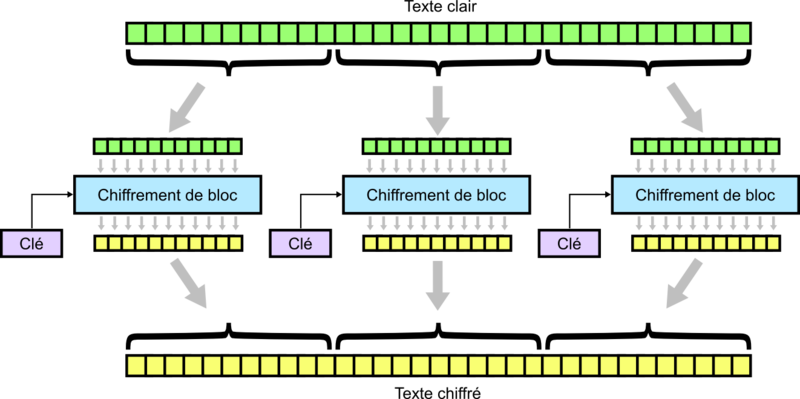
\includegraphics[width=\textwidth]{fonctionnement-ECB}
  \caption{schéma ECB \cite{wiki}}
  \label{schema ECB}
\end{figure}

Ce mode présente les avantages du chiffrement par flots, est pré-calculable et est parallélisable. Il offre la possibilité de déchiffrer une zone quelconque du texte chiffré et ainsi de déchiffrer une partie seulement des données.

Cependant ce mode possède un défaut considérable: deux blocs de texte clair seront chiffrés de la même manière, car il n'y a pas de randomisation. Ce défaut rend le mode ECB vulnérable aux attaques par dictionnaire et à l'analyse fréquentielle. En effet pour une clef donnée, on pourra générer un dictionnaire avec les correspondances entre les clairs et le chiffré, permettant ainsi de retrouver le texte clair. Pour ces raisons l'utilisation de ce mode est fortement déconseillé bien qu'il soit défini par défaut dans de nombreuses applications comme MySQL.

\section{CBC}
\label{cbc}
Avec le mode CBC (Cipher Block Chainning ou Enchaînement des blocs), on applique à chaque bloc de texte clair un "XOR" (ou exclusif) avec le bloc chiffré précédent. Ainsi chaque bloc chiffré dépend des blocs traités auparavant. Pour le premier bloc il faut fournir un vecteur d'initialisation.

\begin{figure}[!h]
  \centering
  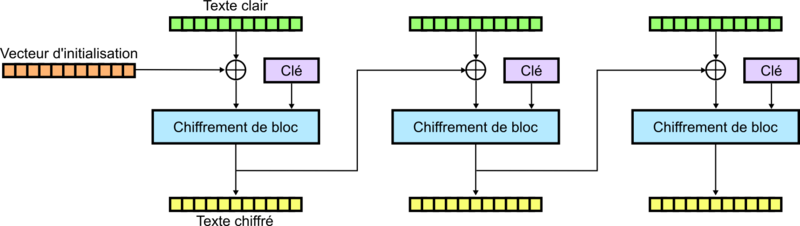
\includegraphics[width=\textwidth]{fonctionnement-CBC}
  \caption{schema CBC - Chiffrement \cite{wiki}}
  \label{schema CBC - Chiffrement}
\end{figure}

Ce mode possède les avantages du chiffrement par flots, et il offre également la possibilité de déchiffrer une zone quelconque du texte chiffré. Cependant un des inconvénients est que le chiffrement est séquentiel ( \cad il ne peut pas être parallélisé).

Pour le déchiffrement, on passe le premier bloc crypté dans le déchiffrement de bloc et on effectue un "XOR" avec le vecteur d'initialisation IV. Dans le cas où le vecteur d'initialisation est incorrect seul le premier bloc crypté sera impossible à décrypter. En effet à chaque bloc on applique un "XOR" avec le chiffré du bloc précédent, et pas le texte clair. Ainsi on peut retrouver un bloc de texte clair uniquement à partir du bloc crypté précédent, ce qui permet ainsi la parallélisation de la décryption. 

\begin{figure}[!h]
  \centering
  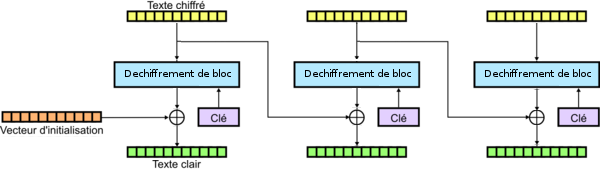
\includegraphics[width=\textwidth]{fonctionnement-CBC_de}
  \caption{schema CBC - Déchiffrement}
  \label{schema CBC - Déchiffrement}
\end{figure}




\section{CFB}
Le mode CFB (Cipher FeedBack ou Chiffrement à rétroaction) est similaire au mode CBC. Tout comme le CBC, ce mode permet de déchiffrer n'importe quelle zone du chiffré. Cependant, comme le CBC, le chiffrement est séquentiel, il ne peut donc pas être parallélise. Le déchiffrement est similaire au CBC et peut, quant à lui, être parallélisé. 

\begin{figure}[!h]
  \centering
  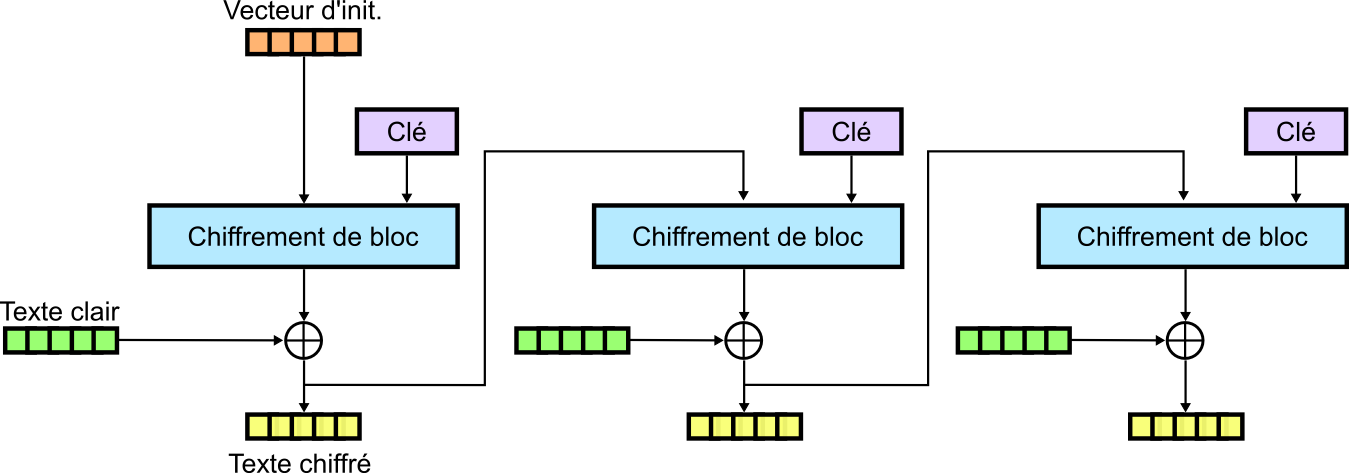
\includegraphics[width=\textwidth]{fonctionnement-CFB}
  \caption{schema CFB - Chiffrement}
  \label{schema CFB - Chiffrement}
\end{figure}

\begin{figure}[!h]
  \centering
  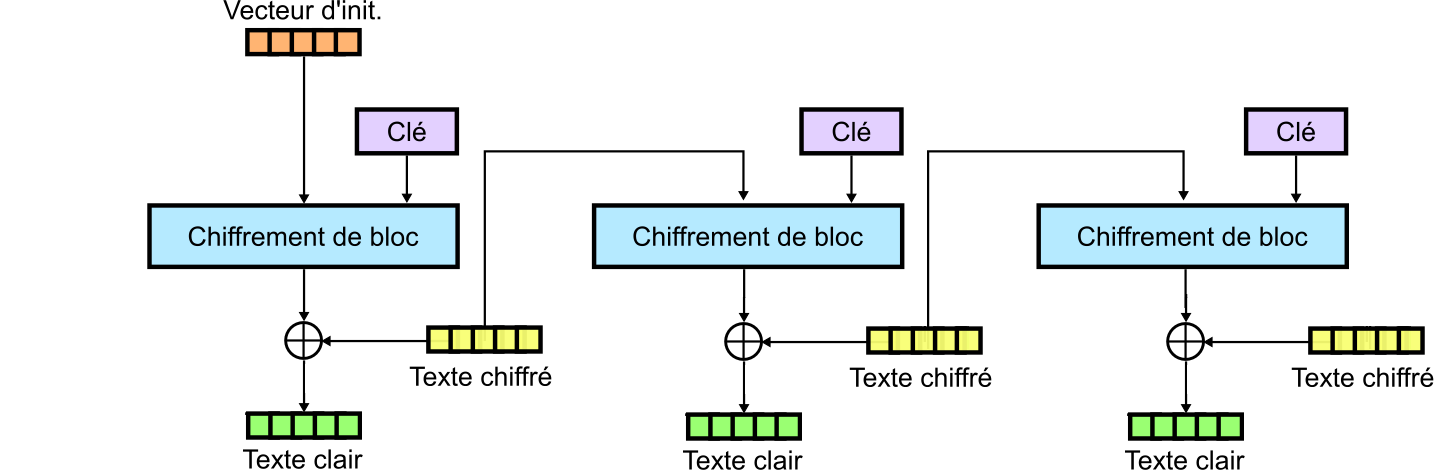
\includegraphics[width=\textwidth]{fonctionnement-CFB_de}
  \caption{schema CFB - Déchiffrement}
  \label{schema CFB - Déchiffrement}
\end{figure}

\section{OFB}
Le mode OFB (Output FeedBack) est une variante du mode CFB. En effet, au lieu d'utiliser un bloc chiffré pour chiffrer le suivant, le mode OFB va utiliser le chiffré du vecteur d'initialisation. S'il s'agit du bloc N, alors celui-ci sera chiffré avec le vecteur d'initialisation chiffré N fois. Le décryptage est très proche du CFB, il faut juste prendre le déchiffré du vecteur d'initialisation.


\begin{figure}[!h]
  \centering
  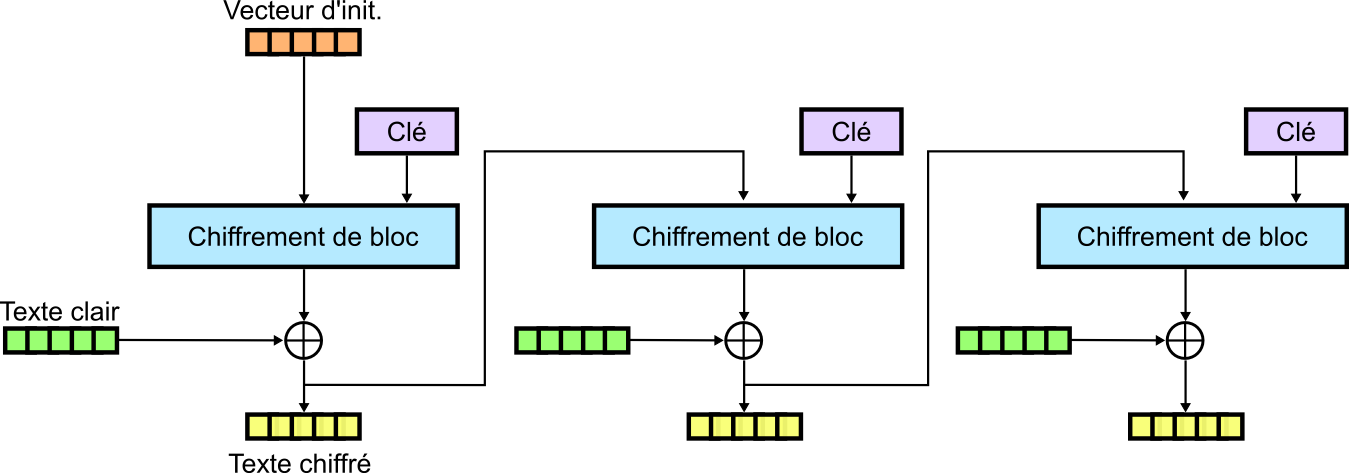
\includegraphics[width=\textwidth]{fonctionnement-OFB}
  \caption{schema OFB - Chiffrement}
  \label{schema OFB - Chiffrement}
\end{figure}

\begin{figure}[!h]
  \centering
  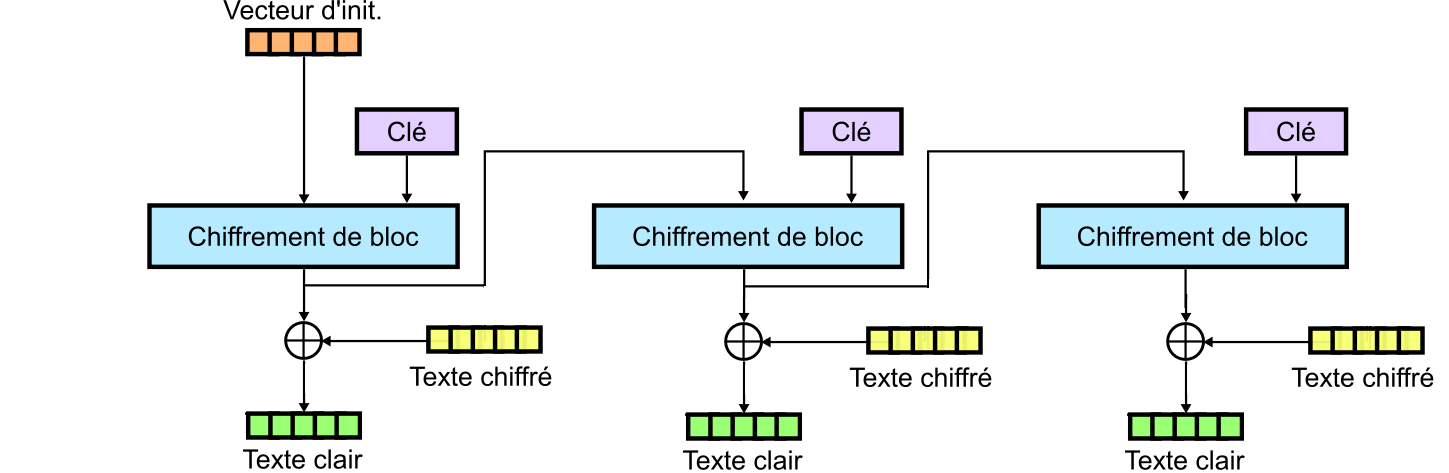
\includegraphics[width=\textwidth]{fonctionnement-OFB_de}
  \caption{schema OFB - Déhiffrement}
  \label{schema OFB - Déchiffrement}
\end{figure}

\section{CTR}
\label{ctr}
%Comme le mode OFB, le mode CTR permet le chiffrement par flot et est pré-calculable. De plus il offre un accès aléatoire aux données, est parallélisable et n'utilise que la fonction de chiffrement. 

Comme on peut le voir sur la figure \ref{schema CTR - Chiffrement}, le mode CTR chiffre un compteur avec une clef (K) à travers un algorithme. Ensuite il réalise une opération de type \og XOR\fg{} (ou exclusif) sur le texte clair avec la sortie de l'algorithme pour obtenir le texte chiffré. 

Comme le mode OFB, le mode CTR combine les avantages du chiffrement par flots, est pré-calculable et est parallélisable. En effet il est possible de calculer à l'avance en parallèle tous les chiffrés des compteurs. Il ne restera plus qu'à les passer dans la fonction XOR avec le clair pour obtenir le chiffré.




\begin{figure}[!h]
  \centering
  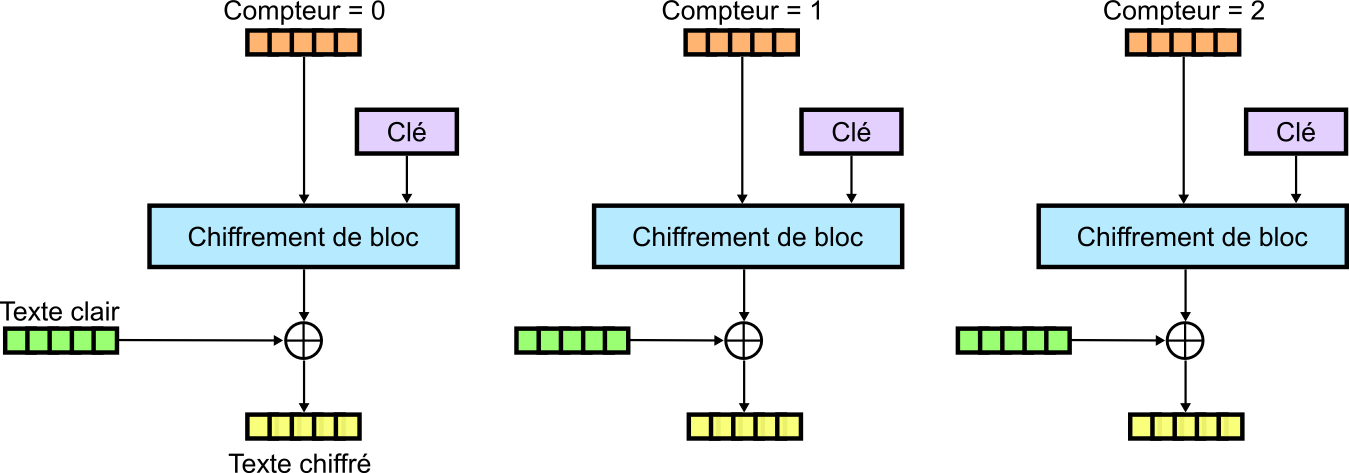
\includegraphics[width=\textwidth]{ctr}
  \caption{schema CTR - Chiffrement \cite{wiki}}
  \label{schema CTR - Chiffrement}
\end{figure}


%%% Local Variables: 
%%% mode: latex
%%% TeX-master: "rapport_de_base"
%%% End: 

\chapter{Les différents modes de fonctionnement de l'AES}
\label{chap:différents modes}

Il existe plusieurs modes de fonctionnenement de l'AES, comme l'\aes. Nous présenterons ici les plus utilisés.

\section{ECB}

Le mode ECB (Electronic codebook ou dictionnaire de code) est le plus simple. Il consiste à diviser le message à chiffrer en blocs qui vont être chiffrés indépendament les uns des autres. Pour le déchiffrement on procédera de la même manière en découpant le texte chiffré en blocs et en décryptant les blocs indépendament les uns des autres.

\begin{figure}[!h]
  \centering
  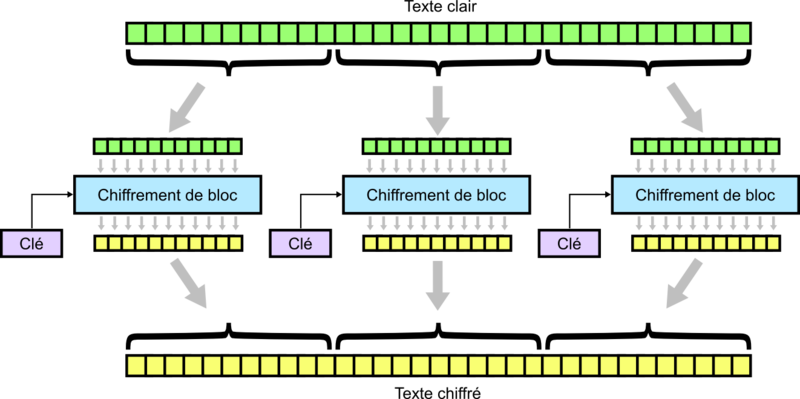
\includegraphics[width=\textwidth]{fonctionnement-ECB}
  \caption{schéma ECB \cite{wiki}}
  \label{schema ECB}
\end{figure}

Ce mode présente les avantages du chiffrement par flots, est pré-calculable et est parallélisable. Il offre la possibilité de déchiffrer une zone quelconque du texte chiffré et ainsi de déchiffrer une partie seulement des données.

Cependant ce mode possède un défaut considérable: deux blocs de texte clair seront chiffrés de la même manière, car il n'y a pas de randomisation. Ce défaut rend le mode ECB vulnérable aux attaques par dictionnaire et à l'analyse fréquentielle. En effet pour une clef donnée, on pourra générer un dictionnaire avec les correspondances entre les clairs et le chiffrés, permettant ainsi de retrouver le texte clair. Pour ces raisons l'utilisation de ce mode est fortement déconseillé.

\section{CBC}

Avec le mode CBC (Cipher Block Chainning ou Enchaînement des blocs), on applique à chaque bloc de texte clair un "XOR" (ou exclusif) avec le bloc chiffré précedent. Ainsi chaque bloc chiffré dépend des blocs traités auparavavant. Pour le premier bloc il faut fournir un vecteur d'initialisation.

\begin{figure}[!h]
  \centering
  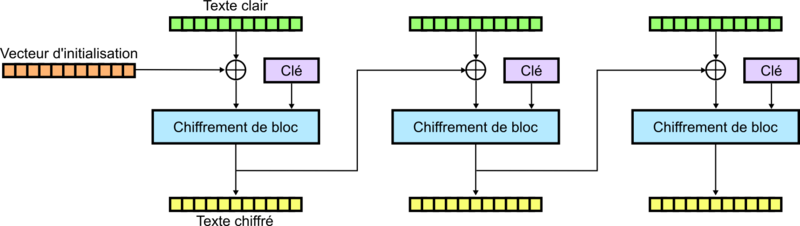
\includegraphics[width=\textwidth]{fonctionnement-CBC}
  \caption{schema CBC - Chiffrement \cite{wiki}}
  \label{schema CBC - Chiffrement}
\end{figure}

Ce mode présente possède les avantages du chiffrement par flots, et il offre également la possibilité de déchiffrer une zone quelconque du texte chiffré. Cependant un des inconvénients est que le chiffrement est séquentiel ( \cad il ne peut pas être parallélisé).

Pour le déchiffrement, on passe le premier bloc crypté dans le déchiffrement de bloc et on effectue un "XOR" avec le vecteur d'initialisation IV. Dans le cas où le vecteur d'initialisation est incorrect seul le premier bloc crypté sera impossible à décrypter. En effet à chaque bloc on applique un "XOR" avec le chiffré du bloc précédent, et pas le texte clair. Ainsi on peut retrouver un bloc de texte clair uniquement à partir du bloc crypté précédent, ce qui permet ainsi la parallélisation de la décryption. 

\begin{figure}[!h]
  \centering
  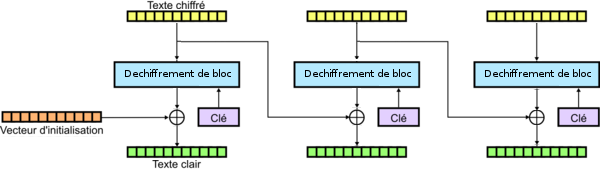
\includegraphics[width=\textwidth]{fonctionnement-CBC_de}
  \caption{schema CBC - Déchiffrement}
  \label{schema CBC - Déchiffrement}
\end{figure}




\section{CFB}
Le mode CFB (Cipher FeedBack ou Chiffrement à rétroaction) est similaire au mode CBC. Tout comme le CBC, ce mode permet de déchiffrer n'importe quelle zone du chiffré. Cependant, comme le CBC, le chiffrement est séquentiel, il ne peut donc pas être parallèlisé. Le déchiffrement est similaire au CBC et peut, quant à lui, être parallélisé. 

\begin{figure}[!h]
  \centering
  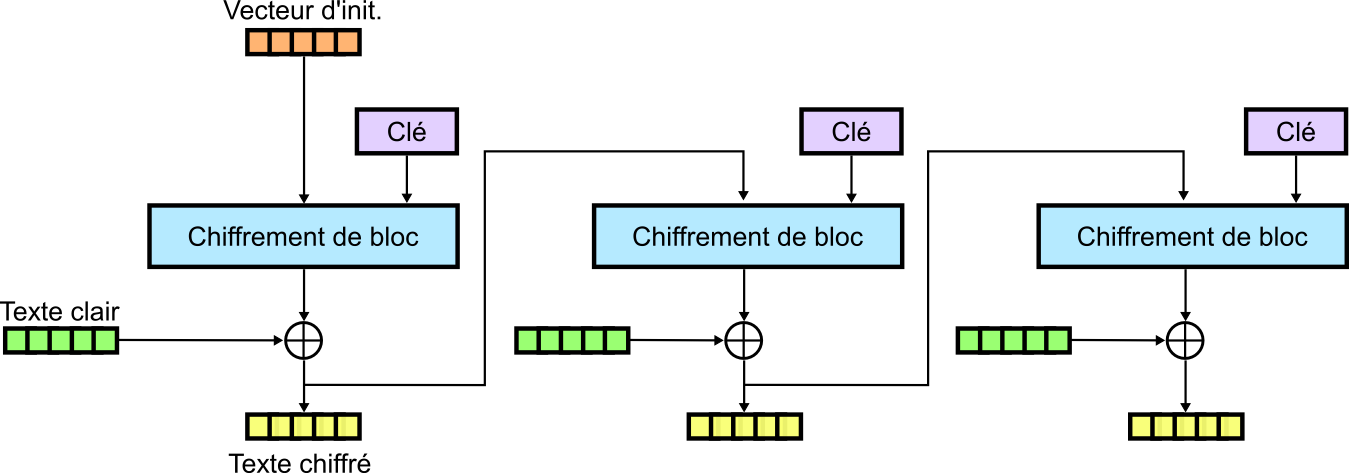
\includegraphics[width=\textwidth]{fonctionnement-CFB}
  \caption{schema CFB - Chiffrement}
  \label{schema CFB - Chiffrement}
\end{figure}

\begin{figure}[!h]
  \centering
  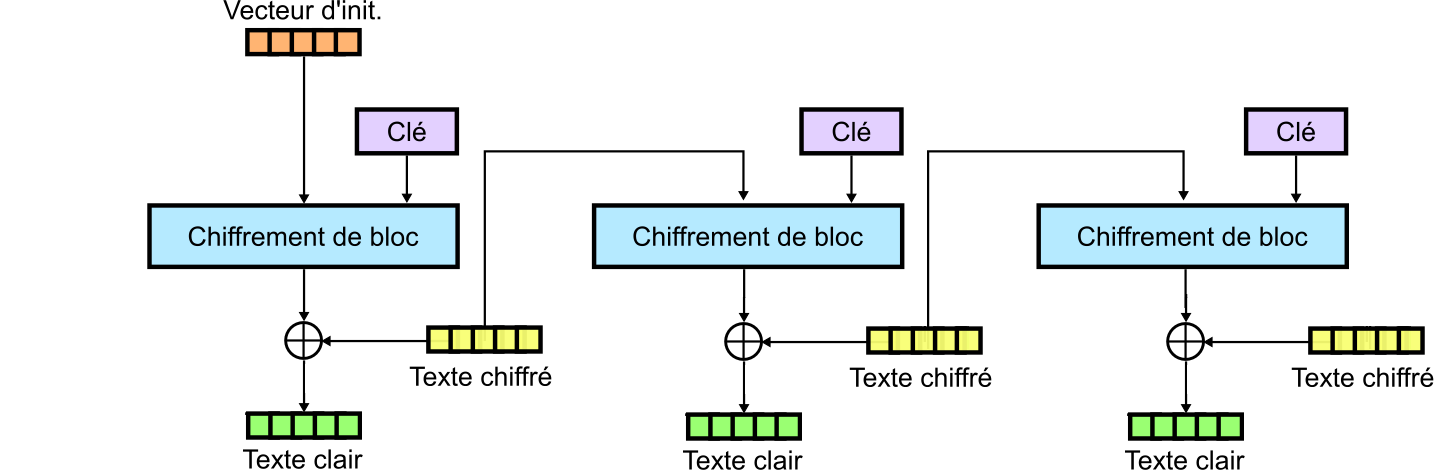
\includegraphics[width=\textwidth]{fonctionnement-CFB_de}
  \caption{schema CFB - Déchiffrement}
  \label{schema CFB - Déchiffrement}
\end{figure}

\section{OFB}
Le mode OFB (Output FeedBack) est une variante du mode CFB. En effet, au lieu d'utiliser un bloc chiffré pour chiffrer le suivant, le mode OFB va utiliser le chiffré du vecteur d'initialisation. S'il s'agit du bloc N, alors celui-ci sera chiffré avec le vecteur d'initialisation chiffré N fois. Le décryptage est très proche du CFB, il faut juste prendre le déchiffré du vecteur d'initialisation.


\begin{figure}[!h]
  \centering
  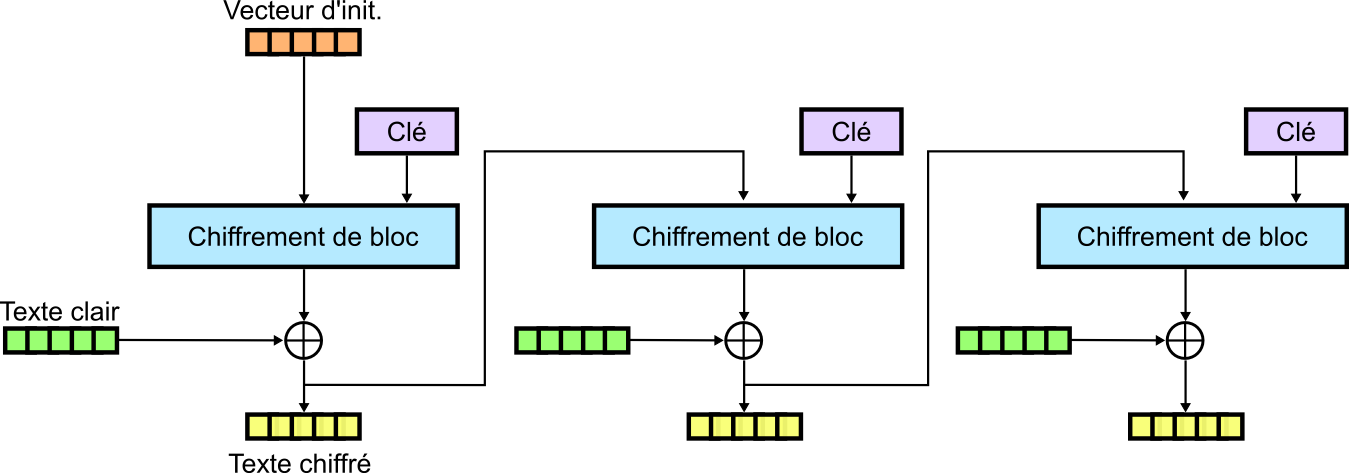
\includegraphics[width=\textwidth]{fonctionnement-OFB}
  \caption{schema OFB - Chiffrement}
  \label{schema OFB - Chiffrement}
\end{figure}

\begin{figure}[!h]
  \centering
  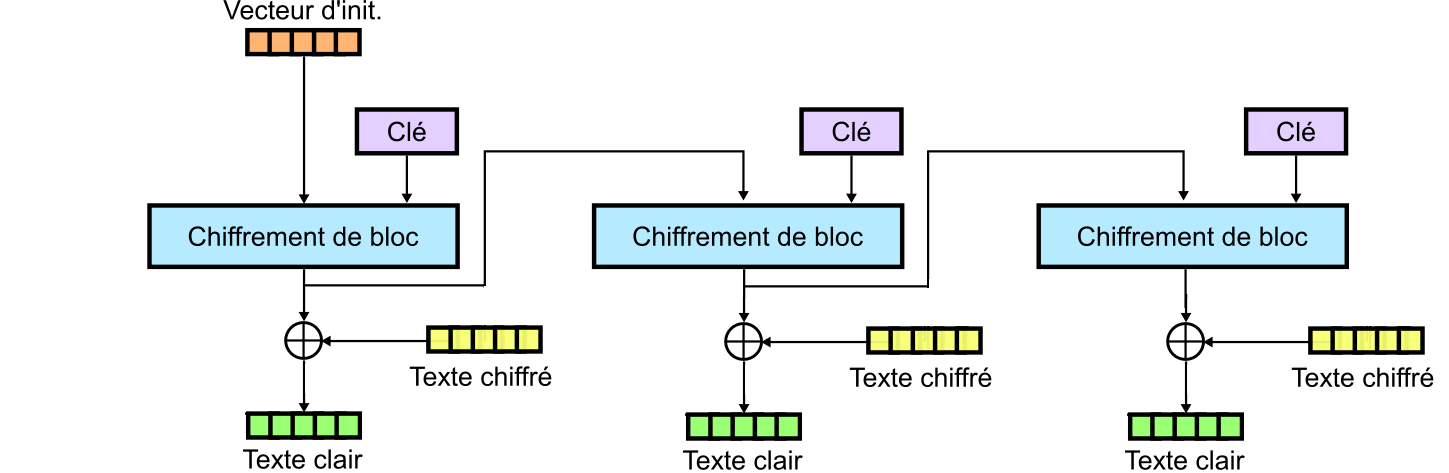
\includegraphics[width=\textwidth]{fonctionnement-OFB_de}
  \caption{schema OFB - Déhiffrement}
  \label{schema OFB - Déchiffrement}
\end{figure}

\section{CTR}
Comme le mode OFB, le mode CTR permet le chiffrement par flot et est pré-calculable. De plus il offre un accès aléatoire aux données, est parallélisable et n'utilise que la fonction de chiffrement. 

\begin{figure}[!h]
  \centering
  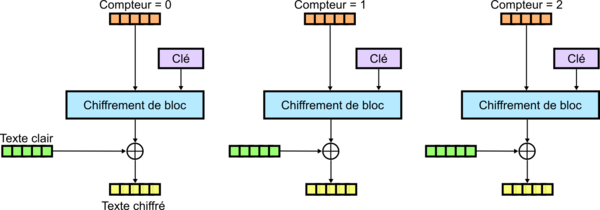
\includegraphics[width=\textwidth]{fonctionnement-CTR}
  \caption{schema CTR - Chiffrement}
  \label{schema CTR - Chiffrement}
\end{figure}


%%% Local Variables: 
%%% mode: latex
%%% TeX-master: "rapport_de_base"
%%% End: 

\chapter{Comparaison GCM - CCM - OCB}

Lors de nos recherches nous avons constaté que les algorithmes fournissant à la foi la confidentialité, l'authenticité et l'intégrité sont: GCM, CCM, OCB, CWC, EAX et APM.

Mais paris eux seulement trois sortent du lot GCM, OCB et CCM. C'est pourquoi nous avons décidé d'écarter les autres algorithmes et de seulement comparer ces trois.

\section{CCM}

Comme son nom le suggère le mode CCM combine le mode CTR et le mode CBC-MAC. C'est deux modes "primitfs" sont combinés pour authentifier les données puis les encrypter. CBC-MAC permet dans un premier temps d'obtenir un tag d'authentification du message clair. Puis le message et le tag sont chiffrés en utilisant le mode CTR.



Le vecteur d'initialisation (IV) doit est être choisi avec précaution car il ne doit jamais être utilisé plus d'un fois par clef. En effet le mode CCM est un dérivé du mode CTR.



Une idée essentielle est que la même clé de cryptage peut être utilisé à la fois pour l'authentification et l'encryptage, à condition que les valeurs de comptage utilisées dans le cryptage ne rentrent pas en collision avec le vecteur d'initialisation (VI) utilisé pour l'authentification.


\begin{figure}[!h]
  \centering
  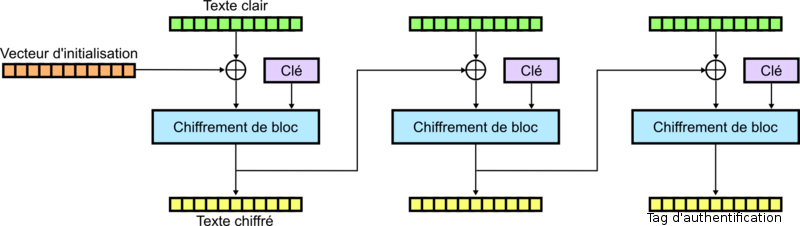
\includegraphics[width=\textwidth]{fonctionnement-CBC_MAC}
  \caption{Création du tag d'authentification avec CBC-MAC}
  \label{Création du tag d'authentification avec CBC-MAC}
\end{figure}

\begin{figure}[!h]
  \centering
  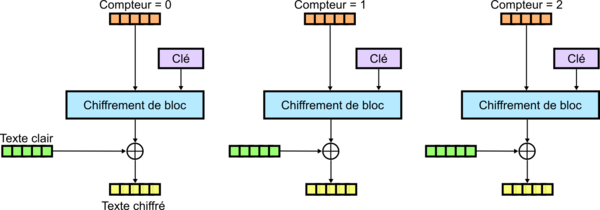
\includegraphics[width=\textwidth]{fonctionnement-CTR}
  \caption{Chiffrement du tag et du message avec CTR}
  \label{Chiffrement du tag et du message avec CTR}
\end{figure}


Contrairement à \aes, la génération du tag d'authentification (via CBC-MAC) est faîte a partir du message en clair et non pas le message encrypté. Au niveau performances, le mode CCM va utiliser de manière général plus de calcul que \aes. En effet dans \aes l'authentification et l'encryption ne font appel qu'a une seule fois au chiffrement AES par bloc tandis que pour le mode CCM va utiliser une première fois le chiffrement AES pour l'encryption puis une seconde fois pour générer le tag d'authentification. De plus le mode CCM ne peut pas être parallélisé.


\newpage


\section{OCB}
Le mode OCB est lui aussi conçu pour fournir à la fois l'authentification et la confidentialité. OCB (Offset CodeBook) est basé sur le mode ECB avec l'utilisation d'un vecteur d'initialisation. Pour l'authentification il faut d'abord effectuer un checksum du message clair, ce checksum est ensuite encrypter comme un block du message clair. 

\begin{figure}[!h]
  \centering
  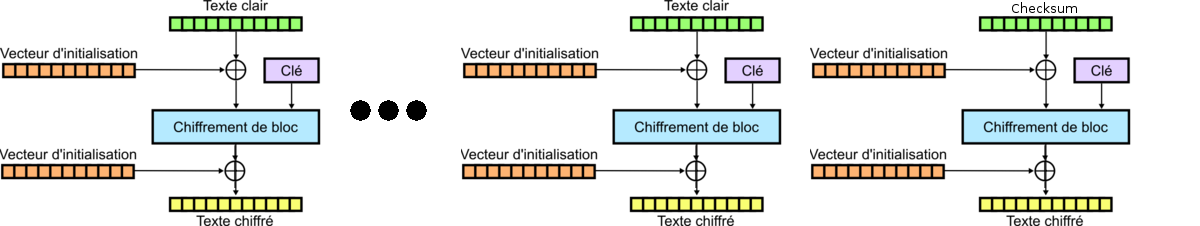
\includegraphics[width=\textwidth]{fonctionnement-OCB}
  \caption{Fonctionnement du mode OCB}
  \label{Fonctionnement du mode OCB}
\end{figure}

AES-OCB est un mode de fonctionnement qui est soumis à deux brevet au Etat-Unis qui empêchent son utilisation dans toute application commerciale ou gouvernementale au Etat-Unis. 
De plus Niels Ferguson a montrer l'existance d'attaque sur le mode OCB qui limite l'envoie de données à 64GB par clef. D'un point de vue performance, le mode OCB est légerement plus rapide que \aes car il ne nécéssite pas l'implementation des multiplications dans l'espace de Galois.


%%% Local Variables: 
%%% mode: latex
%%% TeX-master: "rapport_de_base"
%%% End: 


%%%% CONCLUSION %%%%%%%%%

\chapter*{Conclusion}
\addcontentsline{toc}{chapter}{Conclusion}

Face à cette étude nous pouvons conclure que \aes est un algorithme très puissant et rapide qui permet d'assurer la confidentialité, l'intégrité et l'authenticité des données.

Il est évidemment a recommander par rapport au autres mode d'AES qui n'assure pas l'authenticité. Mais nous avons également vu qu'il fallait privilégier dans l'algorithme GCM l'utilisation de AES par rapport à Treefish ou Salsa20 qui sont bien moins utilisé.

Enfin nous avons constaté que l'utilisation de GCM est bien plus performante que d'autre algorithme comme OCB ou CCM pour réalisé l'authenticité et l'intégrité.


\newpage

%%%% ANNEXE %%%%%%%%%%%%

\part*{Annexe}
\appendix
\nocite{*}

\chapter{Les alternatives à AES}
\label{anexe1}

Nous discuterons dans ce chapitre des alternatives existantes à l'AES. Ces alternatives sont pertinentes car elles pourrait améliorer les performances de \aes sans réduire sa capacité d'authentification et d'intégrité.

\section{Rijndael - Twofish - Serpent}
Rijndael est l'algorithe qui remporta en octobre 2000 le concours AES lancé en 1997 par NIST et devient le nouveau standard de chiffrement. (Advanced Encryption Standard)

Parmis les finalistes, autre que Rijndael, se trouvaient les algorithmes Serpent et Twofish. Ces deux algorithmes sont des algorithmes de chiffrement par bloc qui ont subi de nombreuses analyses cryptographiques. Cependant aucun de ces deux algorithmes n'a reçu beaucoup d'attention depuis l'adoption de Rijndael comme nouveau standard. Les derniers résultats les plus significatifs datent ainsi de 2000. Rijndael s'est imposé comme nouveau standard et est massivement utilisé.

\section{Salsa20}
Salsa20 est un algorithme de chiffrement par flots, contrairement à AES qui est un algorithme de chiffrement par blocs. Cette distinction est importante car un algorithme de chiffrement par flots permet de produire une chaine pseudo-aléatoire de bits auxquels sont appliqués un XOR avec le message à encrypter. Les algorithmes de chiffrement par bloc peuvent être configurés en chiffrement par flots (mode CTR ou OFB).

Comme nous l'avons vu précédement, les algorithmes de chiffrement par blocs peuvent être configurés pour à la fois assurer l'encryption mais également l'authentification. De plus dans la plupart des modes de fonctionnement des algorithmes par blocs on peut accèder à des parties spécifiques du texte crypté.
Salsa20 permet un accès à une partie spécifique de la sortie encryptée. En effet l'algorithme salsa20 a besoin d'une clef, d'un vecteur d'initialisation et d'un numéro de bloc, ce qui lui permet de décrypter n'importe quel bloc.

Il est également possible d'utiliser Salsa20 en mode authentifié, pour cela il faut coupler l'algorithme Salsa20 avec un algorithme d'authentification de messages comme le Poly1305 créé par Daniel J. Bernstein. Le problème est que cet usage n'est pas standardisé.

Un des arguments positifs de Salsa20 est qu'il est rapide en logiciel. L'initialisation et le paramètrage de la clef est négligeable, et il possède un faible nombre de cycles par byte par rapport aux autres algorithmes. En effet Salsa20 peut être 2 à 3 fois plus rapide que AES en mode CTR.

Les principales limitations d'un algorithme comme Salsa20 sont les mêmes que pour tous les algorithmes de chiffrement non-standard: ils sont alternatifs et n'ont ainsi pas la même attention et ne sont donc pas standardisés par des organismes comme NIST. Bien que Salsa20 ait subit un nombre décent d'analyses crypatanalogiques, la plus part positives, ce n'est rien comparé à AES.


\section{Threefish}
Threefish est une contribution récente aux algorithmes alternatifs à AES. Threefish fait partie des algorithmes de chiffrement à avoir réussi la plupart des compétitions organisées par NIST. Threefish est un algorithme de chiffrement par blocs qui peut être configuré pour fonctionner sur des blocs de taille 256, 512 ou 1024 bits. Alors que Threefish a subit quelques cryptanalyses, cela reste encore relativement limité. Aucun de ces travaux n'ont montré de résultats probants quant à une éventuelle faille de sécurité, ce qui inspire plutôt confiance. Encore une fois, les études menées n'ont rien de comparable avec celle faites sur AES, et ainsi il est difficle de dire où se situe Threefish par rapport à AES en matière de sécurité.

%%% Local Variables: 
%%% mode: latex
%%% TeX-master: "rapport_de_base"
%%% End: 

%\input{annexe_}
\newpage
 \listoffigures
 \printindex
 \bibliographystyle{frplain}
  \bibliography{biblio}

\end{document}
%%%%%%%%%%%%%%%%% FIN DU DOCUMENT
